
\title{Recap Computer network technologies and services (01OTWOV)}
\author{Jacopo Nasi\\
        Computer Engineer\\
        Politecnico di Torino}
\date{I Period - 2017/2018\\\bigskip\bigskip\today}

\documentclass[12pt]{article}
\usepackage[utf8]{inputenc}
\usepackage[italian]{babel}
\usepackage{geometry}
\usepackage{indentfirst} % First line indent
\usepackage{mathtools}
\usepackage{wrapfig}
\usepackage[usenames, dvipsnames]{color}
\usepackage{float}
\usepackage{amssymb}
\usepackage{ifsym}
% Misure Documento
\geometry{ a4paper, total={170mm,257mm},left=35mm, right=35mm, top=35mm, bottom=35mm }

\begin{document}

\begin{figure}
  \centering
  
\includegraphics[width=10cm]{images/polito.pdf}
\end{figure}

\maketitle

\newpage
\tableofcontents

\newpage
{\noindent \Large \textbf{License}\bigskip}

This work is licensed under a Creative Commons Attribution-NonCommercial-ShareAlike 3.0 Unported License.\\
You are free:
\begin{itemize}
  \item \textbf{to Share}: to copy, distribute and transmit the work
  \item \textbf{to Remix}: to adapt the work
\end{itemize}
Under the following conditions:
\begin{itemize}
  \item \textbf{Attribution}: you must attribute the work in the manner specified by the author or licensor (but not in any way that suggests that they endorse you or your use of the work)
  \item \textbf{Noncommercial}: you may not use this work for commercial purposes.
  \item \textbf{Share Alike}: if you alter, transform, or build upon this work, you may distribute the resulting work only under the same or similar license to this one.
\end{itemize}

\noindent More information on the Creative Commons website (http://creativecommons.org).

\begin{figure}[h!]
  \centering
  
\includegraphics[width=3cm]{images/license.png}
\end{figure}

{\noindent \Large \textbf{Acknowledgments}\bigskip}

Questo breve riepilogo non ha alcuno scopo se non quello di agevolare lo studio di me stesso, se vi fosse di aiuto siete liberi di usarlo.\\
Le fonti su cui mi sono basato sono quelle relative al corso offerto (\textbf{Computer network technologies and services (01OTWOV)}) dal Politecnico di Torino durante l'anno accademico 2017/2018.\\
Non mi assumo nessuna responsabilità in merito ad errori o qualsiasi altra cosa. Fatene buon uso!
\newpage

\section{IPv6}
\subsection{Why we need another version?}
The main problem of the previous version of IP haven't enough address space for our society. The are other motivations:
\begin{itemize}
  \item More efficent on LANs: You need to use ARP to know the host.
  \item Multicast and unicast
  \item Secutiry
  \item Policy Routing
  \item Plug and Play: IPv4 wasn't created with DHCP.
  \item Traffic Differentiation
  \item Mobility: The position of a mobile device change often.
  \item QoS
\end{itemize}
The great number of the this characteristics are achieve with the older version with less efficency, the real motivation is actually the address space. The transition isn't too easy and an interim solution is needed and it's why the IPv6 isn't already used by everyone like the 4 version.

\paragraph{Lack of IPs} the 32bit address can provide 4 billion of address but not all are available for the CLASS division and only 3.5 billion are still usable. The problem is that when the IPs are assigned an entire class of IP is assigned, in the case of Politecnico the authority give a B class (130.192.xxx.xxx) that it means 65.025 IP address but the reality is that we not need to much IPs and the not used ones are wasted. When the IP started to be used the auth give without paying to much attention at the numbers of wasted address. A similar problem coming from the wasted IP that must have the same prefix to be on the same network, if you have 100 host you will need at least a network of 2\^7 = 128 available IPs but you will wasted the remaing 28 IPs. This is caused because the IPs are used Hierarchically, divided in more part, increasing the hierarchically will means an increase of waste.

\paragraph{Interim solution} during the period fo transition between the two versions we need a continuity, the main solution adopted were:
\begin{enumerate}
  \item Taylored Assignement
  \item Private Address
  \item Network Address Translator (NAT)
  \item Application Level Gateway (ALG)
\end{enumerate}
The authority in charge of distributing the IP address is the IANA that distributes the adr to the regional agencies, if you look at the figure \ref{fig:wastedIP} you can see the distribution of the IPs between the different region. The yellow correspond to not already assigned IP adresses, the purple blue segmente rappresente the \"active\" IPs but the purple part rappresent addresses that aren't available between the router all around the world, this part is really big and it represents all the addresses wasted that we have mentioned before.
\begin{figure}[h!]
  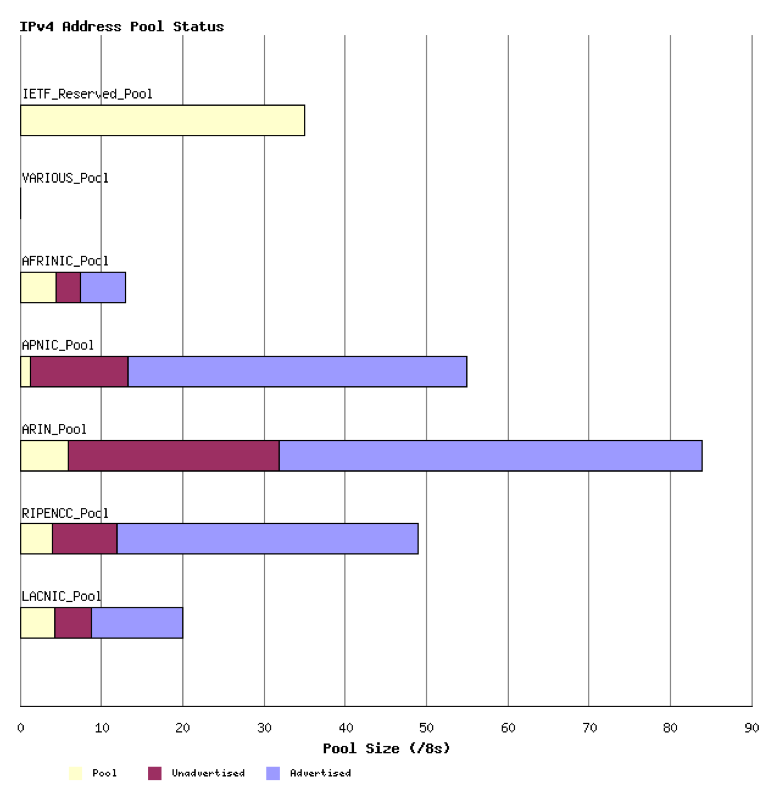
\includegraphics[width=\linewidth]{images/wasteIP.png}
  \caption{IPv4 Pool Status}
  \label{fig:wastedIP}
\end{figure}
% IPv6 block @ Pag. 18

\bibliographystyle{abbrv}
\bibliography{simple}

\end{document}
